
\documentclass[article]{IEEEtran}
\usepackage{graphicx}
\usepackage{float}
 \usepackage{url}
\usepackage{amsmath}
\setlength{\parskip}{0.5em}
\setlength{\parindent}{2em}

\begin{document}

\title{Fundamentals of Artificial Intelligence Assignment 2- Solving the Travelling Salesman Problem with Genetic Algorithms}

\author{\IEEEauthorblockN{Craig Heptinstall}
\IEEEauthorblockA{Crh13- 110005643\\SEM6120\\
Institute of Computer Science\\
Aberystywth University}}

\maketitle

\begin{abstract}
Genetic algorithms provide an optimization technique for a wide variety of problems, including that of the travelling salesman. The number of solutions for a TSP can become exponential, which genetic algorithms such as roulette, tournament and others can help reduce the number of evaluated solutions vastly. 
\end{abstract}

\section{Introduction}
Genetic algorithms are considered in a wide array of problems where exact algorithms would struggle. The travelling salesman problem is a great example of a problem that does not have a means of finding the best solution first time, and would be increasingly time consuming to loop through all possible solutions to find the lowest cost (length of path).

\subsection{Travelling Salesman Problem}
To understand the travelling salesman problem, the reasons for its existence and early sources should be known. The travelling salesman problem was thought up in 1930 \cite{1} by Merrill Flood whilst looking to solve a school bus routing problem. The problem stems off from the Hamiltonian cycle puzzle, requiring the solver to visit all node or ‘cities’ once in a set of \( \mathcal{N} \) cities. At this point in time, no general method of solution is known \cite{2} (so is considered NP-hard) therefore only the best and shortest paths can be evaluated from several attempts. \par
Because of the nature of the problem, genetic algorithms appear as an idealistic means of finding optimised tours where a solution cannot be found using a mathematical means. Evolutionary algorithms used in genetics may never be guaranteed to find optimal solutions, though due to their random nature they will often find a good solution \cite{3}. Genetic algorithms are called as so because of the similar way they act to natural selection, with the best and most efficient parents creating more advantageous children. In the instance of the travelling salesman, this could be reflected where two parents whose path distances are short are combined to form a child who uses similar paths to that of its parents, combined with a small form of randomness in the hope of improving upon a solution. \par
Figures \ref{fig:1} and \ref{fig:2} show an example TSP with a low number of points where an optimal solution can be found quite easily by exact, heuristic or GA means. An important aspect expressed in Figure \ref{fig:2} is that although all the points are visited, the final vertex visited must also be linked to the first in order to return to the starting position.
\begin{figure}
\centering
  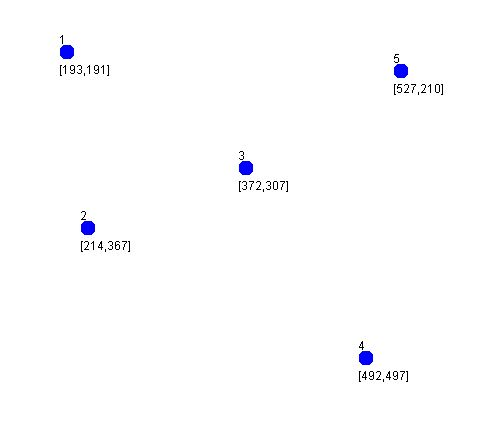
\includegraphics[width=.8\linewidth]{images/problem}
  \caption{An example set of vertices where a travelling salesman problem is present.}
  \label{fig:1}
\end{figure}
\begin{figure}
\centering
  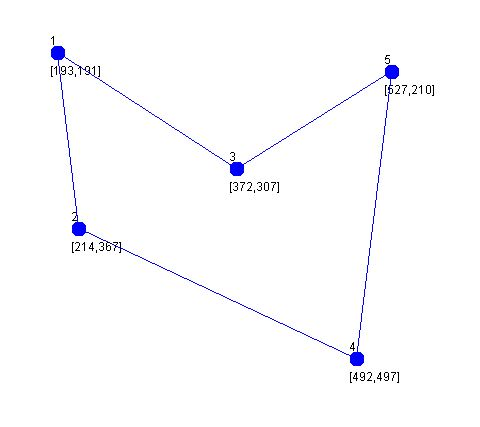
\includegraphics[width=.8\linewidth]{images/solution}
  \caption{A possible solution to the TSP expressed above.}
  \label{fig:2}
\end{figure}

\section{Genetic algorithms considered for TSP}
Before looking at the possible genetic algorithms to be considered for such a puzzle as the TSP, it should be understood that a very basic generic algorithm can be used for such a purpose. In a paper in the Scientific World Journal \cite{4}, a team worked on using a traditional algorithm created back in 1989 by David Goldberg \cite{5} and improving its efficiency to help solve the TSP quickly and as accurately as possible. The original genetic algorithm, which many algorithms are based from today goes through the following process:
\begin{enumerate}
\item Randomly generate an initial population of chromosomes.
\item Use the fitness function to select the fitter chromosomes.
\item Apply the crossover and mutation operators in order. 
\item If a stopping criterion is satisfied, then stop and output the best chromosome
\item Go back to step 2
\end{enumerate}

\section{Proposed solution}
The following sub sections of this paper discusses the merits and drawbacks of using certain genetic algorithm selection strategies. Testing the capabilities of GA's using different means of selecting individual chromosomes (or tour solutions in the case of the travelling salesman problem) will allow statics and conclusions to be applied to the respective strategies, and have a higher chance of finding best possible results for the TSP problem. Alongside selection, the concept of elitism is looked at. Elitism may prevent strong solutions being lost on mutation and crossover, and therefore create better, faster-found routes. 

\subsection{Considered and selected GA representations}
As already discussed in the previous section of the paper, most GA's have been based off of older ones such as chromosome representation \cite{5}. For the purpose of this paper, the algorithm used for the TSP will be also based on this algorithm though different aspects such as crossover, mutation and elitism types will be looked at. To keep the algorithm at a simple chromosome state will allow easier implementation of the algorithm in code form, therefore will be easier to manipulate and change specific aspects to allow for statistical research. \par
There are three parts of the genetic algorithm that will be heavily considered in this paper, each of which will be modified and replaced by other means to compare and find the most optimal solutions to the travelling salesman problem. The three which are integral to any good GA, and which will be explained the need for in the TSP in the following sections are:
\begin{enumerate}
\item Selection- Selects two 'parents' from the current population, usually picking two strong chromosomes is ideal in order to ensure a strong 'child' is created. This like nature, as the strongest usually survive and again produce offspring which inturn makes the population stronger as a whole.
\item Crossover- The algorithm responsible for mating the two parents selected in the previous state of the GA. By mixing the two parents as efficiently as posisble, two strong child chromosomes should be created using traits from both parents. 
\item Mutation- Once the population has been updated with its new chromosomes formed from previous solutions, there should be some small amount of mutation to some of the the chromosomes. This allows the random chance that the solution could get better in some cases, therfore when selected and mated again the overall population may get better.
\end{enumerate}
Each of these components of the GA to be used in the application will be descirbed in the following section, each of which provided alongside how the application could implement them.

\subsubsection{Selection methods}
In order to create the most efficient child chromosomes (or path around TSP nodes in this case), there a range of availible algorithms that can be used to select parent chromosomes. There are subcategories of selection stratedgies which are explained in some depth on Marek Obitko's 'Introduction to genetic algorithms' \cite{6} . The first of which should be explored is the simple but effective roulette wheel selection technique. This works by imagining all the solututions are placed as roulette wheel numbers, with each solution having a proportion of the wheel decided by its fitness value. \par
A radnomly genertaed number between zero and the total fitness of the population is then selected, and starting with the chromosomes with the higher fitness values, there fitness is subtracted from the random number until that number equals or is below zero. This process stops and the that chromosome is returned as a parent. This could be compared to the roullette ball stopping on a track. \par
By having the roulette wheel broken up by the size of fitness values, the larger the fitness value means the better chance of being selected. When a random number is selected, Figure \ref{fig:3} shows how some chromosomes could be placed onto a roulette wheel system. 
\begin{figure}[H]
\centering
  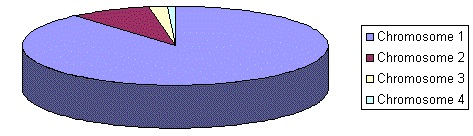
\includegraphics[width=.8\linewidth]{images/rouletteWheel}
  \caption{A roulette wheel example showing a single chromosome with a far better fitness than the others.}
  \label{fig:3}
\end{figure}
To implement this into a TSP solver application, this will be done by simply looping through all of the paths, getting a total fitness and then looping again deducing each fitness value until zero is reached. This will be the simplest of the algorithms to implement and should be made to be built upon for other such algorithms like rank based ones. \par
The issue with roulette selection which is solved by the second selection method whcih will be used by a proposed TSP solver applicaation is that if there is a clear best chromosome with a fitness value that differs largly from the others then its chance of getting selected to be a parent may be two high, therefore childs formed may always be from parents which are the same. This defeats the purpose of the crossover. \par
To solve this, a function called rank selection was created to keep in mind that although chromosomes with better fitness should have a higher chance of being selected, but they should have more of an exponential system to keep chances fair. Therefore, rank based system simply assigns the best fiteness chromosome with a higher standard number, and this number is decreased as the rank of each chromosome is less. For example, with a population of 5, the best chromosome would be assigned the rank 5, and the next 4 and so on. This then means that although the roulette ball will still have the possibibilty of landing on any chromosome, the chances of landing on higher and lower fiteness chromosomes wil be biased more fairly. Figure \ref{fig:4} shows an example rank system in use with a set of chromosomes.
\begin{figure}[H]
\centering
  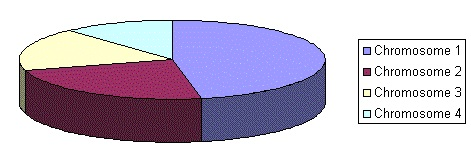
\includegraphics[width=.8\linewidth]{images/rank}
  \caption{An improved form of the roulette wheel with a fairer system of laying out chromosomes.}
  \label{fig:4}
\end{figure}
In the case of this TSP solver application, this could be done by firstly comparing each of the path lengths in the population, and then ordering them by lowest fitness first. Once this is complete, a fitness can be assigned to each starting with the population size, and decreasing the value of the fitness by one with each iteration. Once they are ranked, the roulette wheel method can use the edited population.\par
The third and final selection technique to be explored that will be tested in a TSP solver application will be tournament selection method. This uses a different mechanism to the previous two, by only evaluating a given number of solutions in a population rather than the entire population. Using the defined number of randomly selected chromosomes, the algorithm then gets the fitness of each and returns the winning chromosome. The tournament selection method ensures that weaker chromosomes do not make it through to the next evolution. In the case of the proposed application, this would be a simple implementation of a method which takes a population, a requested tournament size, and then uses a random number generator to select solutions before competing them together to return a winner. 

\subsubsection{Crossover methods}
The next integral part of the genetic algorithm to be implemented is the crossover type. For this, two methods have been considered; ordered and uniform. Alike the previous section, both will be discussed how they function and how they will be integrated within the solver application. \par
The reason for only selecting two crossover methods stems from the reason that although many crossover algorithms exist, many of them are inconsistant a probelm such as travelling salesman. For instance, take the crossover example in Figure \ref{fig:5}, after a simple one-point crossover, although the chromosomes have been mixed, the solutions in the childs are no longer valid since not all the points will be visited. A paper by Kylie Bryant which looks at both general genetic algorithms and how they can be applied to the travelling salesman problem mentions that algorithms should be made to make sure that children chromosomes do not finish as illeagle solutions, and that 'in this way, crossover is very problem specific' \cite{7}. \par
The first to be considered is ordered crossover. The same paper explains this type of crossover well, explaining that this type of crossover is very similar to the PMX (partially mapped crossover) method, except instead of repairing chromesomes which contain repeat nodes, the rest of the nodes are rearranged to provide a leagal path. In the application, this will be implemented by starting with a switch of part of two chromosomes between two crossover points. With this complete, then the child chromosomes will be constrcted using genes from the start of the second crossover point, and these are to be  added until the parent is looped over and reach the first crossover point. Finally the selected crossover genes will be placed into the child chromosomes in the position of the first crossover point.
The second crossover algorithm 

TODO!!!!!!!!!!!!!!!!!!!!!!!!!!!!!!!!!!!!!!!!!!!!!!!!!!!!!!!!!!

\subsubsection{Mutation methods}
For the same reason that crossover options are limited due to the NP-Hard nature of the travelling salesmane problem, only a short amount of availible mutation types were availible for consideration. For the purposes of this paper and the application constructed, only one mutation type will be used, swap mutation. Swap mutation is a very ideal solution to mutating points along a TSP becuase it allows routes to branch off and explore paths gradually further down the route as more optimum solutions are found. One author of an online article exploring a similar problem to this paper, states that using simple swap mutation makes the GA 'unable to achieve an optimum quickly but can prevent convergence into a local optimum' \cite{8}. \par
In order to allow the TSP solver to have the best chance of finding optimal solutions wth greater amounts of nodes or cities, the application will use the simple swap mutation algorithm. For instance, in the case that there are fourty points in a TSP, a more advanced swap mutation might find a solution it believes optimal quickly due to little improvement after a certain amount of time, this swap mutation will continue looking at other options and could find a better ending solution. In the results stage of this paper, especially when combined with roulette selection, that the avergage fitness should derease to a low point and then waver at that point until the application stops.\par
The suggested implimentatoin of mutation should involve looping through each city in a path, and selecting two random points, swapping them both. Of course a mutation rate will be set to ensure that swapping is not always performed, otherwise the local minimum fitness may never be found. To do this in terms of programming the solver, a simple check would only allow a swap i the mutation rate is higher than a random number generated between 1 and 0.

\subsubsection{Evolution stop criteria}
The final part of any GA and one that has been considered while planning the implementation the TSP solver is deciding when to stop the evolutions of chromosomes, or in otherwords stopping the looping of selection, crossover and mutation. In a chapter from the book 'Advances in Artificial Intelligence – SBIA 2004' \cite{9}, the three most commonly and widley used stopping criteria are described:
\begin{itemize}
\item An upper limit for number of generations is reached
\item An upper limit on the number of evaulated fitness functions is reached
\item The chance of significant improvement is reached
\end{itemize}
For the purpose of the research in this paper, the first will be implemented in order to allow more flexibility when testing and to allow the user to increase the runtime in order to compare the time required for each selection and crossover to hit a local minimum. This will also provide the ability to run more stressful testing to the algorithms such as increasing the number of cities to larger numbers.

\subsection{Application structure}
Folllowing the completion of research into various implementation options for different parts of the TSP solver application, the structure of the application itself can be detailed. In order to do this, a high level class diagram, alongside a description of communication between classes has been provided in Figure \ref{fig:5}. The language chosen for this implimentation was Java, for its extensive library collections and vast amount of tutorials similaly using the language for other genetic algorithm examples.
\begin{figure}[H]
\centering
  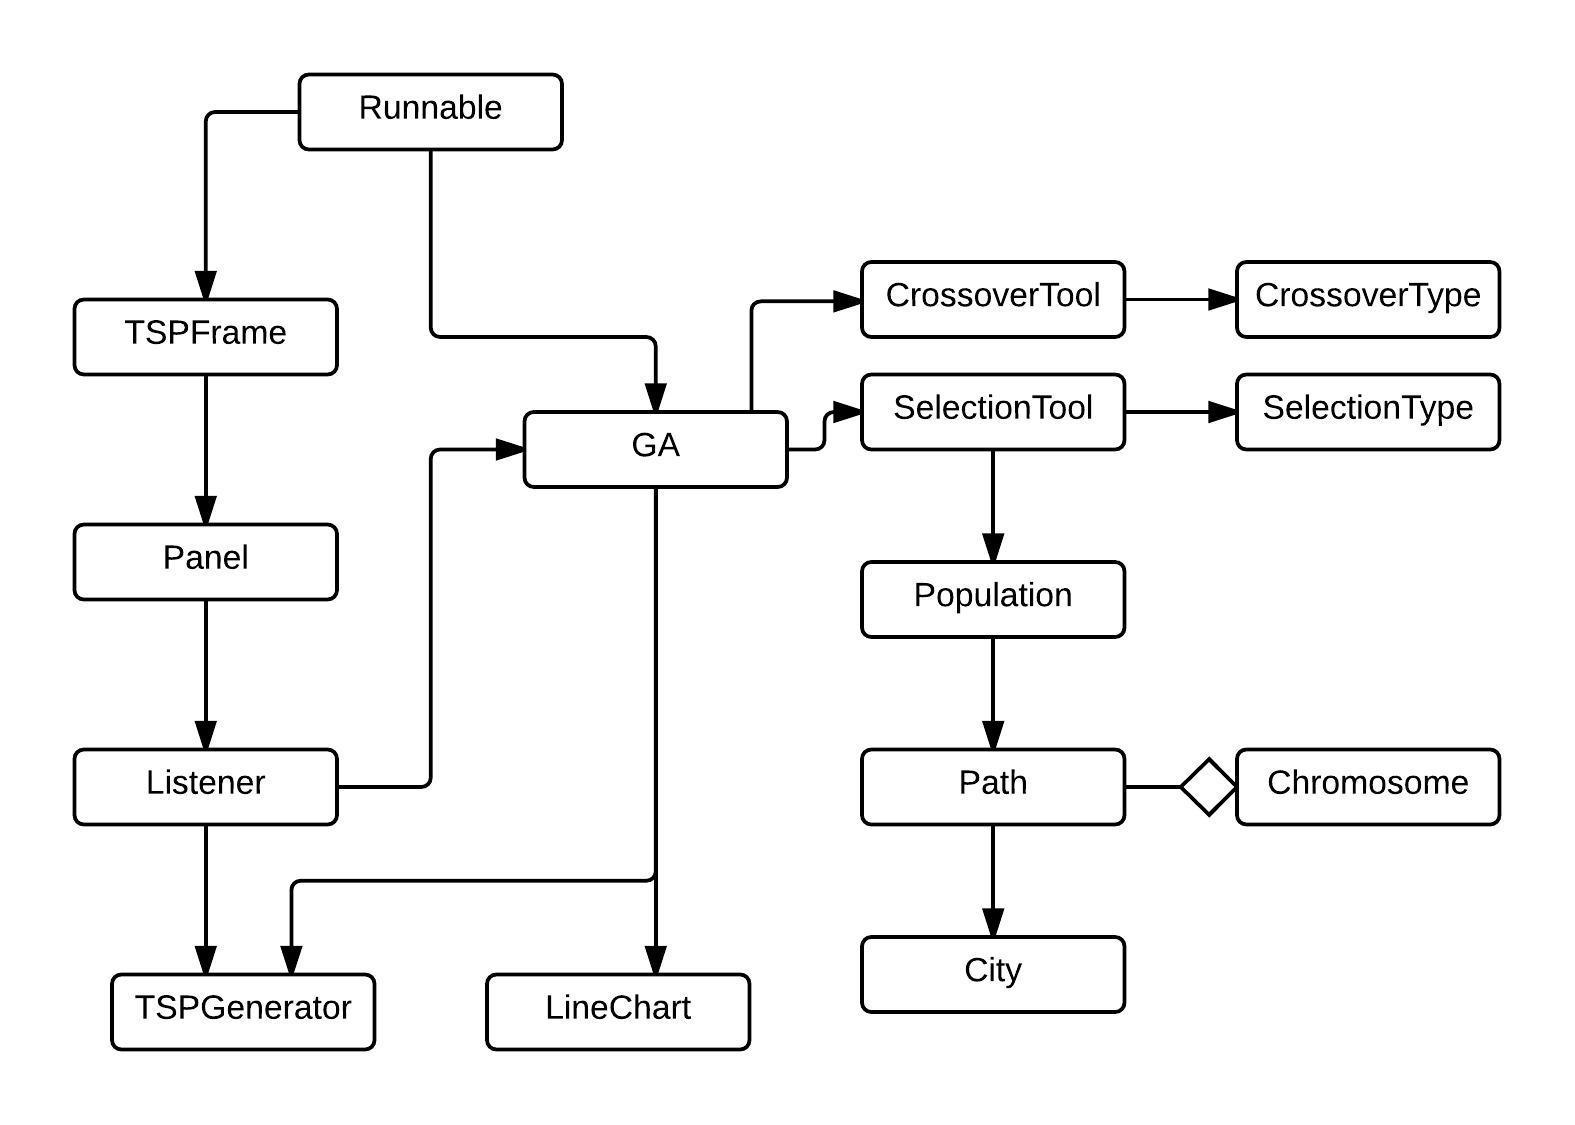
\includegraphics[width=.8\linewidth]{images/class}
  \caption{High level class diagram of the TSP solver application.}
  \label{fig:5}
\end{figure}
As it can be seen in the diagram, there is a GUI in the design which is seperated from the main logic of the application. This was done in order to allow a user wanting to run the application without the front end and opt for the option to use it as a console application only. The application has been made in an object orientated form as much as possible, such as creating objects for cities, paths, and types of crossover/ selection. \par
Starting by looking at key classes in Figure \ref{fig:5}, the main class 'Runnable' is responsible for triggering a run of the algorithm or trigger the opening of the GUI. If the user runs the jr using the 'java' command and passes correct arguments, then the output is printed to the command line alongisde an export of the result csv file, and graphs from runtime. Otherwise the applcation frame is opened, and the user can perofrm actions through controls availible. \par
To keep the GA class as simple as posisble, a lot of the logic for performing the solving of TSP's was placed into helper classes such as selection and crossover 'tools'. Both these classes contain all th implemented methods for crossovers and selections, and are selected via enumerted types for both respectably. All of the algorithms implemented can be found in the previous subection of this paper, and all have graphical and command line options to use each. \par
The TSP generatot class is especially important, making use of teh Java Secure Random library to give less chance of duplicated points. This class has the ability to import and export paths to CSV and is used when the user generates points in the GUI (exporting points), or used when running the application through the command line (reading points in).\par
A quick mention should be made to an extra feature implimented, which allows the user to click anywhere on the canvas to add a new city. This is very useful for testing, as harder, more custom paths can be made. \par
As for represntations of the actual paths, it was ensured that both chromosomes (paths), and genes (cities) would be done in the most object orientated way possible. As shown in the class diagram in Figure \ref{fig:5}, a population is a collection of Paths, with each of these extending an abstract class of type chromosome. This has been done to show the relationship to genetics that the GA has. Within each path, a collection of cities (which represent genes) form the solutions to the given TSP. \par
Other than the GA workings and GUI, there is also a connection to a class 'LineChart'. This class is responsible for generting statistics and graphs of each runtime, from average fitness to lowest distance of a GA. For this, a Java library named jFreeChart \cite{10} was used to save time creating graphs allowing more time for concentrating on the GA. By creating graphs in runtime dynamically, it meant that the next secton of tis paper makes use of statistics already in a well presented form.\par
As with any good appliocation, the TSP solver created is well commented, and Javadoc is availible in the 'dist/Javadoc' folder.

\subsubsection{Running the application}
There are two simple ways of running the application, both through the runnable Jar file. Figure \ref{fig:6} shows the result of simply opening the Jar to open up the GUI. The other option is shown in Figure \ref{fig:7} by running the Jar through the command line to produce a command line repsonse. The primary parameters for this are: name of csv file containing coordiantes; a mutation rate; an evolution amount; whether elitism should be enabled; a selection type; and a crossover type. It should be noted that in order to run the command line version, the GUI version may need to be run if the user wishes to make use of the random point generation operation, which will only export to CSV whilst run in the GUI.

\begin{figure}[H]
\centering
  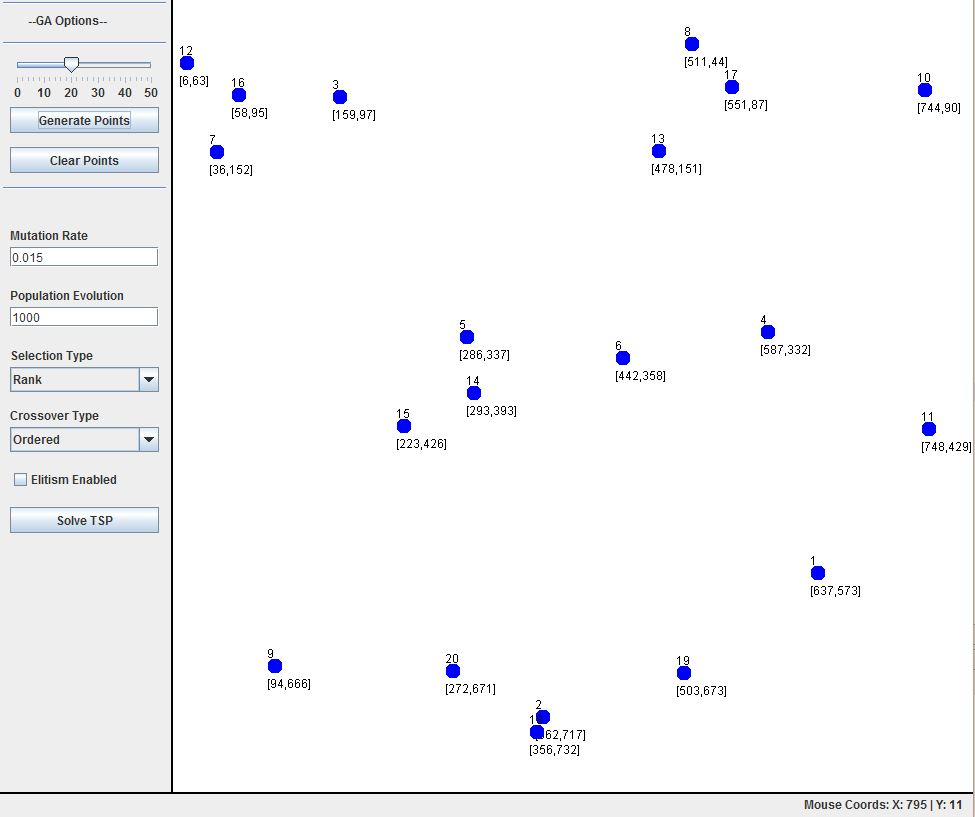
\includegraphics[width=.8\linewidth]{images/GUI}
  \caption{The appplication running with it GUI.}
  \label{fig:6}
\end{figure}

\begin{figure}[H]
\centering
  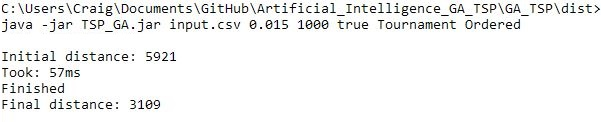
\includegraphics[width=.9\linewidth]{images/commandLine}
  \caption{Example run of the console with example parameters. Output of ordered cities is placed into 'output.csv' file.}
  \label{fig:7}
\end{figure}

\subsection{Comparison of application results}
Using the produced application, a comparison of results from using the different lgorithms implemented can be completed. There will be a range of different test set ups here, all of which will have graphs and statistics attahced, to help compare and decide the best set up for the travelling salesman problem in terms of a genetic algorithm.


\section{Overall findings and conclusion}

\subsection{Improvements to proposed solution}

\begin{thebibliography}{9}

\bibitem{1} 
E.L. Lawler, \textit{The Traveling salesman problem : a guided tour of combinatorial optimization},
1985

\bibitem{2} 
E.W. Weisstein, \textit{Hamiltonian Cycle},
\textit{\url{http://mathworld.wolfram.com/HamiltonianCycle.html}}, 2015

\bibitem{3} 
D.W. Dyer, \textit{When are Evolutionary Algorithms Useful?},
\textit{\url{http://watchmaker.uncommons.org/manual/ch01s02.html}}, 2008

\bibitem{4} 
C.W. Tsai, S.P Tseng, M.C. Chiang, C.S. Yang, T.P. Hong, \textit{A High-Performance Genetic Algorithm: Using Traveling Salesman Problem as a Case},
The Scientific World Journal Volume 2014, 2014

\bibitem{5}
D.E. Goldberg, \textit{Genetic Algorithms in Search, Optimization, and Machine Learning},
Addison-Wesley Longman Publishing Co., 1989. 

\bibitem{6}
M. Obitko, \textit{Introduction to Genetic Algorithms, Selection},
University of Applied Sciences. Czech Technical University., 1998. 

\bibitem{7}
K. Bryant , \textit{Genetic Algorithms and the Traveling Salesman Problem},
Department of Mathematics. Harvey Mudd college., 2000. 

\bibitem{8} 
K. Boukreev, \textit{Genetic Algorithm and Traveling Salesman Problem},
\textit{\url{http://www.generation5.org/content/2001/tspapp.asp}}, 2001.

\bibitem{9}
M. Safe , \textit{On Stopping Criteria for Genetic Algorithms},
Advances in Artificial Intelligence – SBIA 1004., 2004. 

\bibitem{10} 
Object Refinery Limited, \textit{JFreeChart},
\textit{\url{http://www.jfree.org/jfreechart/download.html}}, 2013.

\end{thebibliography}
\end{document}


